\documentclass[11pt,a4paper]{article}
\usepackage[english]{babel}
\usepackage[T1]{fontenc}

\usepackage{amsmath}
\usepackage{amsfonts}
\usepackage{amssymb}
\usepackage{fancyhdr}
\usepackage{a4wide} % Smaller margins = more text per page.
\usepackage[hidelinks]{hyperref}
\usepackage{graphicx}
\usepackage{epstopdf}
\usepackage{pdflscape}
\usepackage{multirow}
\usepackage{subcaption}
\usepackage{bbm}
\usepackage{color}
\DeclareMathOperator*{\argmax}{arg\,max}
\newcommand{\ml}[1]{\textcolor{red}{ML : #1}}
\pagestyle{fancy}
\begin{document}
\author{F\'elix GONTIER \\ \texttt{felix.gontier@ls2n.fr}}
\title{CENSE - Perceptual test II}
\maketitle

\section{Introduction}

This report presents the results of a perceptual experiment conducted as part of the Cense project~\footnote{\url{http://cense.ifsttar.fr/}}. From recordings of a sensor network with low information content, this study aims at proposing a processing chain for the estimation of pleasantness in urban sound environments.

\section{Test description}
\subsection{Objectives}
\label{sec:test_obj}

The objectives of this test are three-fold. First, the study aims at verifying the hypothesis that recorded and equivalent replicated sound scenes result in the same perceptual response, meaning that the development of models based on simulated data for real-life scenarios is feasible.\\

Very few recorded scenes are fully annotated in terms of backgrounds, event onsets-offsets and sound levels. At the same time, the prediction of source-specific acoustic indicators through deep learning models requires large amounts of data for which the ground truth of these indicators is known. An alternative to the subjective annotation of corpora of sound scenes is the use of fully simulated scenes, where source activity is controlled. It is therefore important to verify that new simulated scenes generate a perceptual space similar to that of real scenarios, even with low source complexity.\\

Next, this work aims at finding physical indicators that can be considered for the estimation of pleasantness. Previous studies consistently model pleasantness as a function of perceptual source activity descriptors such as the time of presence. These quantities are somewhat closer to the physical properties of the scene than the more abstract concept of pleasantness. This work thus primarily focuses on the relation of perceived source activity with physical indicators which can be predicted using deep learning architectures.


\subsection{Data}
\label{sec:test_data}

With respect to the three discussed objectives, a test corpus is created based on recordings from one of the four soundwalks studied in~\cite{aumond2017}. The scenes correspond to 19 locations in the 13th district of Paris. For each recording 45 seconds of audio in a single channel are extracted that represent well the properties of their respective ambiances, and without single events overwhelming their overall perception.
The first objective requires the comparison of perceptual assessments for recorded and replicated sound scenes. The original recordings from 6 locations (P1, P3, P4, P8, P15 and P18) with diverse environments are picked to explore different real-life situations, as a function of the classifications proposed in~\cite{gloaguen2017}: \textit{parks}, \textit{quiet street}, \textit{noisy street} and \textit{very noisy street}. For the second part of the corpus sound scenes are simulated based on the 19 45~s extracts. The recordings are first annotated in terms of the following properties:

\begin{itemize}
\item Background sources that are present throughout the whole scene, and are associated with a sound level.
\item Events characterized for each occurrence by their source type, onset-offset and event-to-background ratio (EBR) in dB.
\end{itemize}

The 19 scenes are then replicated using simScene~\cite{rossignol2015} with a database of extracts from recordings of isolated sound sources. This database is constructed from part of the LibriSpeech~\cite{panayotov2015} corpus for voices and Freesound\footnote{\url{https://freesound.org}} contributions for all other sources. For this experiment, the playback sound level is the same as during recordings of the reference scenes, and ranges from 63.9~dB to 79.4~dB.\\

\begin{figure}[!h]
    \centering
    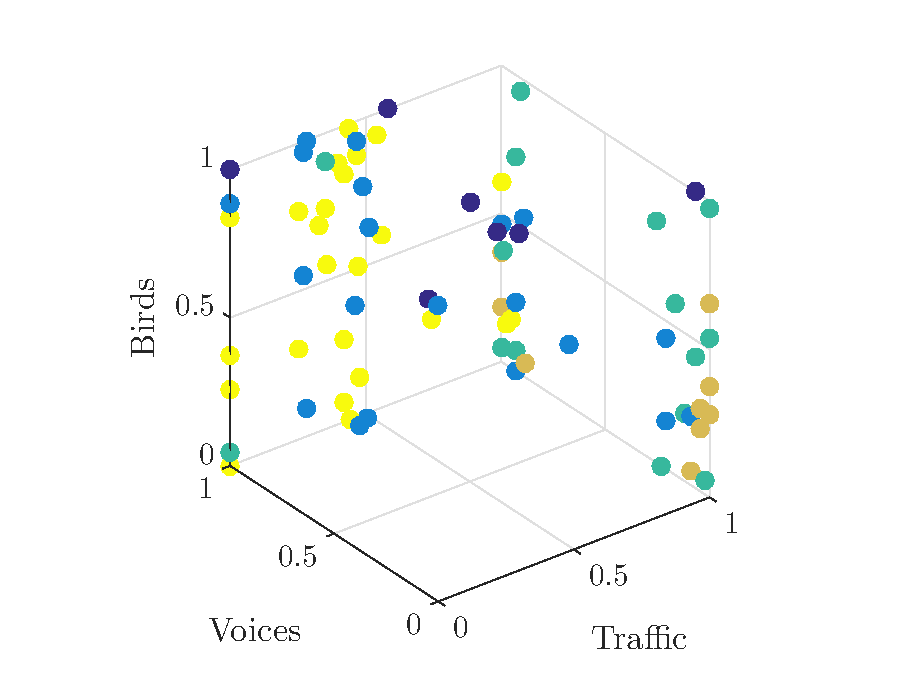
\includegraphics[width=0.6\textwidth]{figures/tvb_pres.eps}
    \caption{Estimated time of presence space for simulated scenes.}\label{fig:tvb_pres}
\end{figure}

To study the perceptual properties of simulated scenes, the corpus is extended with 75 simulated scenes from new scenarios. Because of the lack of large isolated sources datasets, we choose to restrict the scene composition to 3 sources: \textit{traffic}, \textit{human voices} and \textit{birds}. Considering the aim of the study, newly generated scenarios should cover most real-life situations while remaining perceptually plausible. Thus, statistics on background and event properties are extracted for each of the three sources from annotations presented in~\cite{gloaguen2017}. These statistics include, conditionally to the ambiance:
\begin{itemize}
\item The probability of appearance of a given source in the scene, for which events and backgrounds are considered separately,
\item Event-to-background ratios in dB for all events and backgrounds besides the first, in the form of normal distributions,
\item The inter-onset of event occurrences in seconds, also in the form of normal distributions.
\end{itemize}
Adjustments are made on the variance of the considered properties to better cover possible scenarios, and voice events EBR, mostly read English recordings, are reduced to improve realism. An additional \textit{place} ambiance is added with properties derived empirically from available data. For each environment diverse new scenarios are generated by sampling the background and event properties distributions. For each scene the time of presence for the three sources is estimated using indicators proposed in~\cite{gontier2018}, and 75 scenes are chosen to maximize pairwise distance in the resulting 3-dimensional space. This is shown in Figure~\ref{fig:tvb_pres}. The playback sound level is also conditioned on the ambiance according to Figure~\ref{fig:amb_levels}, and ranges from 46.6~dB to 77.1~dB.\\

The experiment corpus totals 100 scenes.

\begin{figure}[!h]
    \centering
    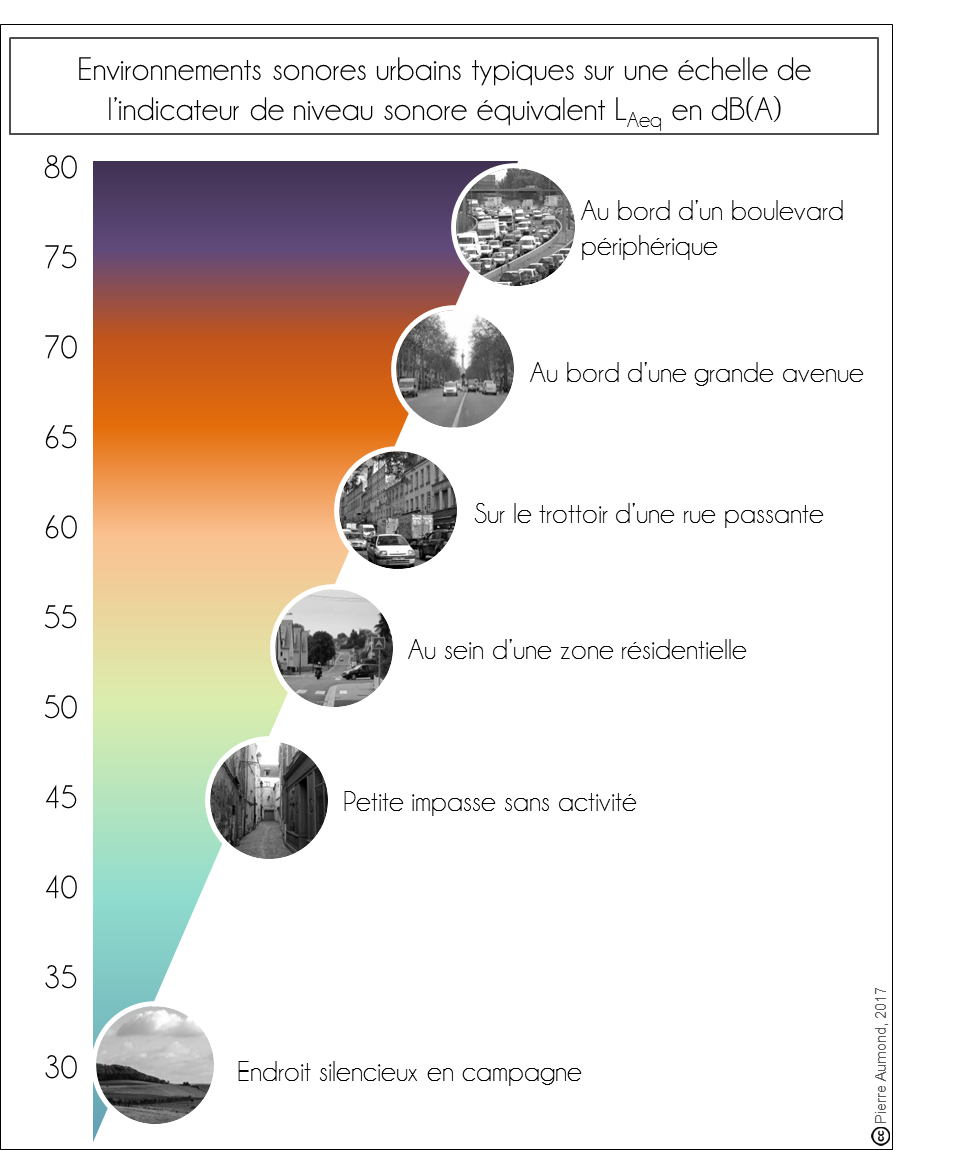
\includegraphics[width=0.4\textwidth]{figures/leqa.png}
    \caption{Scale used to generate sound levels as a function of the environment for new simulated scenes.}\label{fig:amb_levels}
\end{figure}


\subsection{Questions}

Test participants are asked to answer 9 questions per sound scene in the form of 11 point (0-10) scales. They are presented in french and translated in this report using standard terminology. The first 5 scales relate to general properties of the scene:
\begin{itemize}
\item Pleasantness (\textit{Unpleasant - Pleasant}) - P
\item Liveliness (\textit{Inert, amorphous - Lively, eventful}) - L
\item Overall loudness (\textit{Quiet - Noisy}) - OL
\item Interest (\textit{Boring, uninteresting - Stimulating, interesting}) - I
\item Calmness (\textit{Agitated, chaotic - Calm, peaceful}) - C
\end{itemize}
These quantities are typically studied in the perceptual characterization of sound scenes~\cite{axelsson2010, aumond2017, nilsson2007}. While this work focuses on pleasantness, including other dimensions can be useful to verify the relevance of the data in relation to previous work.\\
Furthermore, the primary aim of this test is to model pleasantness from source-specific parameters. Previous studies show that pleasantness is mainly influenced by the activity of three sources: traffic, human voices and birds. The perception of source activity can be linked to notions of dominance, time of presence,  or emergence. We choose the perceptual time of presence, that is the percentage of time for which the corresponding source is heard, as the activity descriptor for this study. The influence of traffic on pleasantness can be different for background and emergent events. Thus, 4 additional questions are presented:
\begin{itemize}
\item Sound level of passing vehicles (\textit{Very low - Very high}) - $L_{T, p}$,
\item Time of presence of Traffic, Voices, Birds (\textit{Never - Continuously}), resp. $T_{T, p}$, $T_{V, p}$ and $T_{B, p}$
\end{itemize}
The corresponding interface is shown in Figure~\ref{fig:interface}.

\begin{figure}
    \centering
    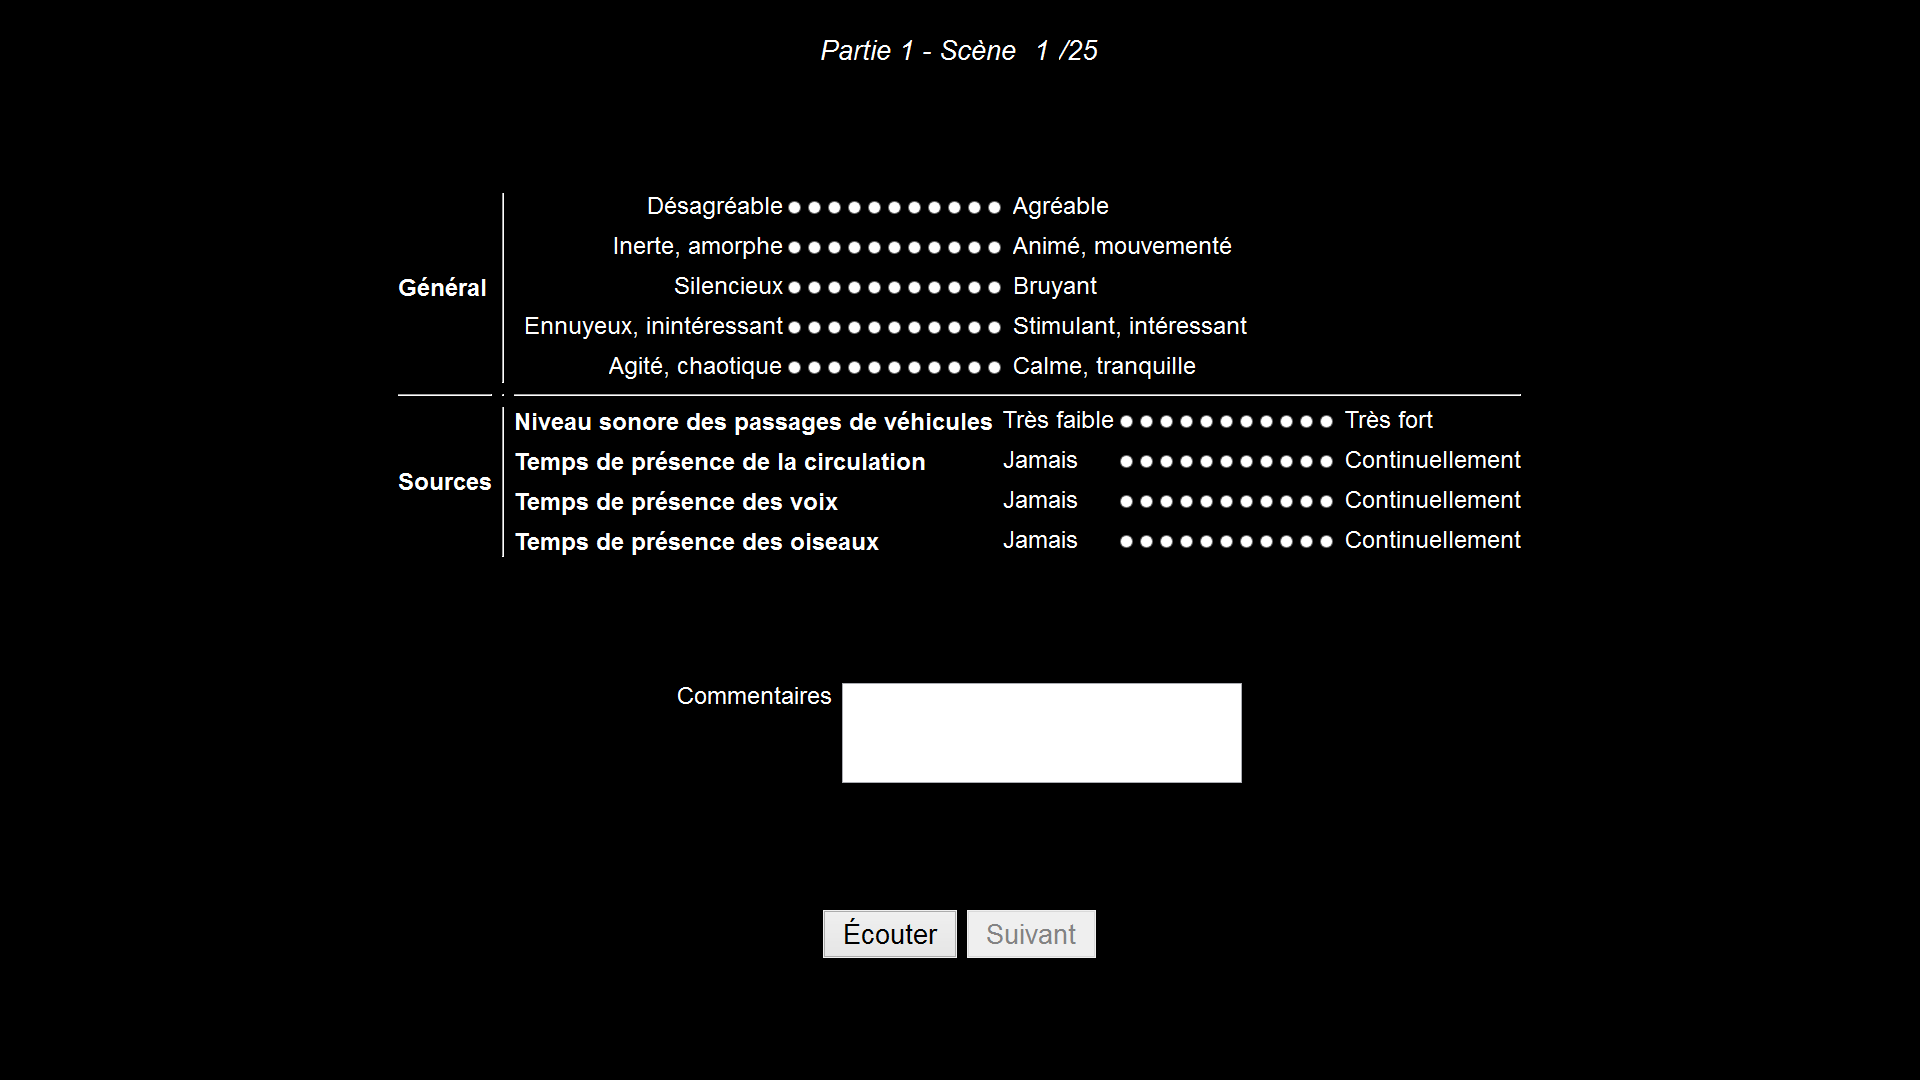
\includegraphics[width=0.9\textwidth]{figures/interface.png}
    \caption{Screenshot of the test interface used by all participants.}\label{fig:interface}
\end{figure}

\subsection{Test conditions}

Prior to the test, participants are given a short verbal introduction and the interface is introduced before the test to ensure that the quantities are well understood. Although the corpus is comprised of 100 sound scenes, participants only evaluate 50 scenes: all listen to the 6 recorded and 19 simulated, then to 25 of the 75 simulated. The evaluated simulated scenes are chosen so that each scene is evaluated by the same number of participants. A random pre-generated order is used to attenuate ordering effects, although all participants are first presented with the most quiet then most noisy of the recorded scenes to calibrate their answers. For the remainder of the corpus all participants experience different scene ordering. Participants can only listen to each scene once. They can start answering questions before the end of the sample, but have to answer all questions and listen to the full extract before proceeding to the next.\\

The scenes are played at a given sound level as discussed in Section~\ref{sec:test_data}, through the same computer and sound card configurations. Beyerdynamics DT-990 Pro headphones are used for all participants. These headphones are calibrated in a semi-anechoic chamber, resulting in a relation between playback Leq and LAeq and sound card output voltage for pink noise. This ensures that correctly scaled scenes will be heard at the desired sound level for all participants.\\

A total of 23 students at Ecole Centrale de Nantes completed the test.

\section{Perceptual analysis}

This section studies the test results with regard to the objectives presented in Section~\ref{sec:test_obj}.\\

Participants evaluate each scene on criteria coded on 10-point discrete scales. Many statistical tools assume that the studied data follows continuous, single mode distributions. It is thus important to first verify that no distinct groups of participants can be obtained from perceptual assessments. A hierarchical clustering analysis of the participants is performed for the 25 scenes in the commonly evaluated sub-corpus, and shown in Figure~\ref{fig:hclusters}. No clear separation into groups is found, as a result the assessment distributions are assumed to be single-mode and their means can be used for further analysis.

\begin{figure}[!h]
    \centering
    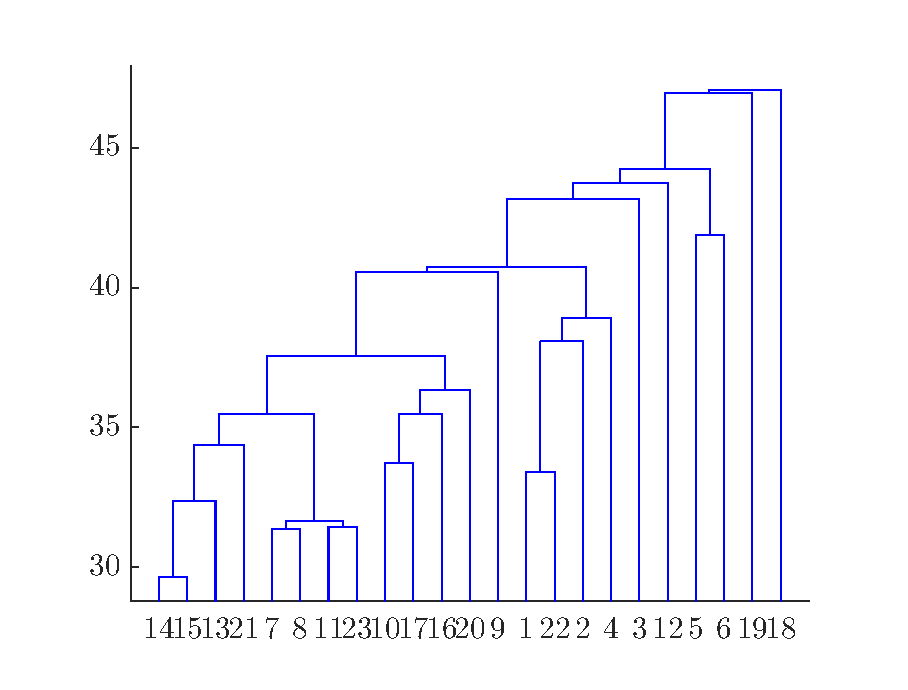
\includegraphics[width=\textwidth]{figures/subj_gr.eps}
    \caption{Dendrogram of the hierarchical clustering of participants on the first 25 scenes of the test. No distinct groups are visible.}\label{fig:hclusters}
\end{figure}

\subsection{Correspondence between recorded and replicated scenes}

The relevance of the remaining study relies on the perceptual equivalence of recorded and synthetic scenes. To verify this hypothesis, the 6 recorded and corresponding replicated scenes are compared in terms of perceptual responses.\\

Table~\ref{tab:ogrep} shows the mean differences between assessments for the recorded and corresponding replicated scenes. Kolmogorov-Smirnov statistical tests are implemented for each scene and perceptual scale to outline significant differences between assessment distributions, which are shown in bold. This non parametric test is chosen because it assumes that distributions are continuous. Pleasantness is found to differ between the two groups only for one location, P4, which can be explained by high discrepancies in the perceptual time of presence of traffic and voices. For this location, the background traffic in the recorded scene varies along time, it is louder in the first half of the scene than in the second half. Replicating this scene using simScene imposes a constant sound level for background sources. Thus, the background traffic is louder in the replicated scene than it is in the recording for about half
of its duration. To a lesser extent the same issue explains the large difference in assessed time of presence of voices in the location P3, but as voices have a less distinct influence on pleasantness this is not reflected directly. Differences can also be interpreted by the choice of isolated samples, which is semi-random and based on a high-level source taxonomy. For example, no difference is made during annotation between child or adult speech, or depending on its expressiveness.\\

Overall, most perceptual responses for replicated scenes are close to those for recordings. No major difference is found in a particular scale, and the proposed hypothesis that recorded and replicated scenes generate the same perceptual responses cannot be invalidated.

\begin{table}[h]
\centering
\caption{Mean differences of perceptual assessments between original and replicated sound scenes. Significantly different distributions as per a Kolmogorov-Smirnov test are in bold (n=23, p<0.05)}
\label{tab:ogrep}
%\resizebox{\columnwidth}{!}{
\begin{tabular}{ c | c c c c c c c c c }
\hline
	 & P & L & OL & I & C & $L_{T, p}$ & $T_{T, p}$ & $T_{V, p}$ & $T_{B, p}$ \\ \hline
	P1 & 0.43 & \textbf{-1.65} & -1.04 & 0.43 & 0.13 & -0.91 & 0.39 & -2.09 & 0.61 \\
	P3 & 0.26 & -0.43 & 0.30 & -1 & 0.30 & 0.35 & 1.04 & \textbf{-4} & 0.22 \\
	P4 & \textbf{0.91} & 0 & \textbf{-1.83} & 0.48 & 1.30 & -0.96 & \textbf{-5.22} & \textbf{1.43} & 0.04 \\
	P8 & 0.26 & \textbf{-1.65} & -0.87 & -0.96 & 0.65 & \textbf{-2.04} & -0.91 & 0.09 & \textbf{-1.43} \\
	P15 & -1.35 & 0.52 & 0.52 & -1.17 & 0.09 & 0.61 & 0.13 & \textbf{1.96} & \textbf{-2.74} \\
	P18 & 1.13 & -0.30 & -1.17 & -0.43 & 1.39 & -1.04 & -1.83 & 0.83 & \textbf{1.30} \\ \hline
\end{tabular}
%}
\end{table}



\subsection{Perceptual space}

The perceptual space generated by the five general scales can also be studied and compared to previous studies to further validate the test material. It is obtained by performing a principal components analysis (PCA) on the corresponding perceptual responses at the scene level. Figure~\ref{fig:pspace} compares the results for scenes based on recordings (left, n=25) and new scenarios (right, n=75). The generated spaces are similar, with only overall loudness and pleasantness axes slightly rotated between the two corpora. For both sets the variance explained by the first two components is similar (resp. 79.4\% - 18.1\% and 79.6\% - 15.2\%). Furthermore, these representations are comparable to those found in previous work on perceptual dimensions~\cite{axelsson2010, cain2013}. Thus, the use of simulated scenes based on both real and new scenarios does not result in major differences in the relations between perceptual quantities. This confirms that the simulation process generates perceptually convincing scenes and can be used for further research.\\

Additionally, assessments for each scene are projected onto the PCA space and represented in Figure~\ref{fig:pspace} as dots. Discrepancies between projections of original and replicated scenes are highlighted in Figure~\ref{fig:pspace}a by black segments. The space covered by scenes based on new scenarios covers that of the studied real-life environments, demonstrating the efficiency of the scene generation procedure in terms of diversity.

% FIGURE
\begin{figure}[h]
    \centering
     \begin{subfigure}[t]{0.5\textwidth}
        \centering
        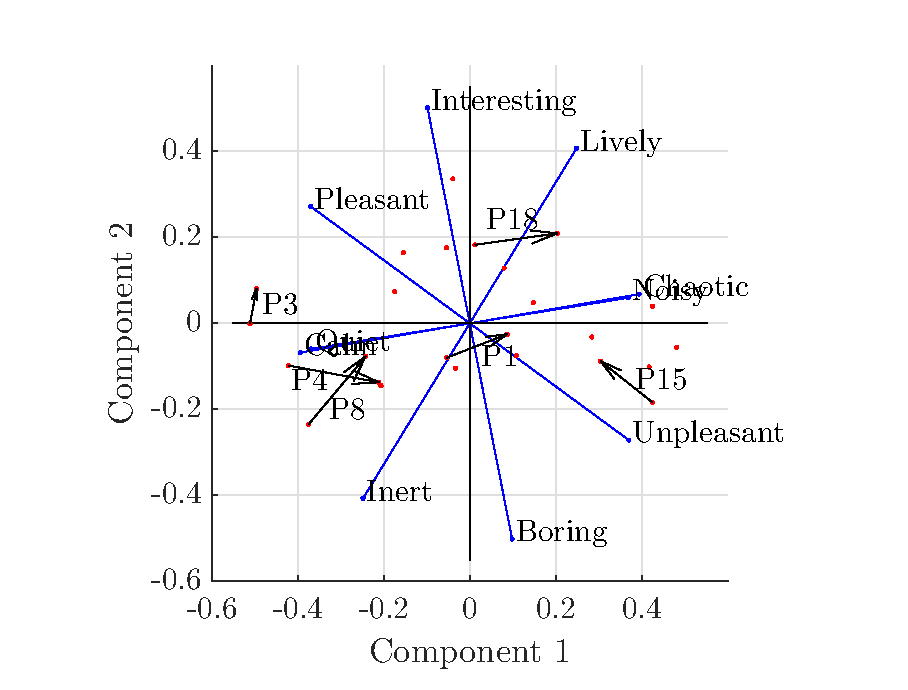
\includegraphics[width=\textwidth]{figures/pca_rep.eps}
    \end{subfigure}%
    \begin{subfigure}[t]{0.5\textwidth}
        \centering
        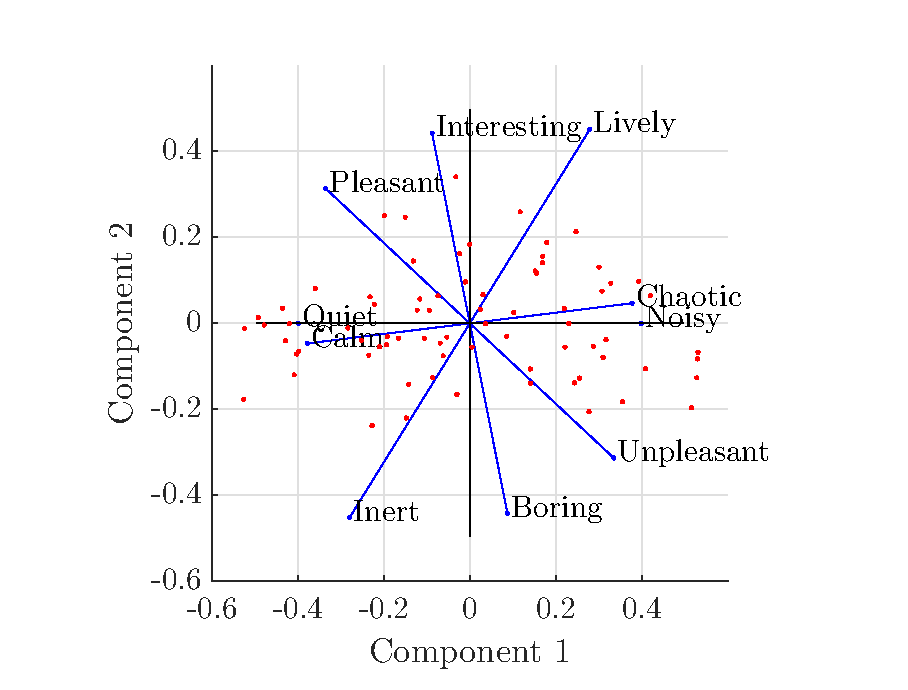
\includegraphics[width=\textwidth]{figures/pca_sim.eps}
    \end{subfigure}
    \caption{Principal components analysis (first two components) of the four general questions at the assessment level (n=252). Each dot represent the projection of one scene on the resulting space. The components space is distorted compared to the litterature.}\label{fig:pspace}
\end{figure}



\subsection{Perceptual scales relationships}
\label{sec:percm}

\begin{table}
\centering
\caption{Pearson's correlation coefficients between perceptual scales at the scene level (n=100, *: p<0.05, **: p<0.01)}
\label{tab:percc}
%\resizebox{\columnwidth}{!}{
\begin{tabular}{ c | c c c c c c c c c }
\hline
	 & P & L & OL & I & C & $L_{T, p}$ & $T_{T, p}$ & $T_{V, p}$ & $T_{B, p}$ \\ \hline
	P & 1 & -0.53** & -0.89** & 0.66** & 0.88** & -0.82** & -0.76** & 0.05 & 0.57** \\
	L &  & 1 & 0.76** & 0.06 & -0.78** & 0.39** & 0.17 & 0.60** & -0.36** \\
	OL &  &  & 1 & -0.39** & -0.96** & 0.71** & 0.59** & 0.17 & -0.45** \\
	I &  &  &  & 1 & 0.35** & -0.55** & -0.67** & 0.38** & 0.48** \\
	C &  &  &  &  & 1 & -0.67** & -0.55** & -0.24* & 0.48** \\
	$L_{T, p}$ &  &  &  &  &  & 1 & 0.79** & -0.15 & -0.41** \\
	$T_{T, p}$ &  &  &  &  &  &  & 1 & -0.35** & -0.42** \\
	$T_{V, p}$ &  &  &  &  &  &  &  & 1 & -0.21* \\
	$T_{B, p}$ &  &  &  &  &  &  &  &  & 1 \\ \hline
\end{tabular}
%}
\end{table}

We then study the relations between perceptual scales with respect to existing work. Table~\ref{tab:percc} shows the Pearson's correlation coefficients at the scene level, that is on the mean responses for each scene. The resulting values are consistent with the literature~\cite{aumond2017, gontier2018}, both between general scales as discussed in the previous section and for the relations to source contributions. Pleasantness (P) is mainly influenced negatively by overall loudness and traffic and positively by birds. In previous studies a small positive contribution of voices to pleasantness was found, while no direct relation is visible from the data gathered. This can be explained by the choice of speech samples used during generation, which consist of read audiobooks extracts and thus may sound unnatural in the considered urban environments. Liveliness (L) is here negatively though weakly (r<0.4) correlated with the presence of birds, while no significant relation was found in previous studies.\\

Relations between source-specific parameters are also weak with the exception of traffic being negatively correlated with birds. The perceptual assessment of the sound level of passing vehicles $L_{T, p}$ is a potential alternative to that of the time of presence of traffic $T_{T, p}$. Except for the interest (I) it displays higher correlations with general scales and lower correlations with other source-specific parameters.\\

To further compare this experiment's results to previous work, multilinear models of pleasantness are built as a function of both the overall loudness (OL) source-specific parameters. To ensure that no multi-collinearity is present between predictors a variance inflation factor (VIF) test is performed prior to model regression. Only models for which all predictors verify $VIF<5$ are considered valid.\\

The best resulting models with statistically significant estimates ($p<0.05$ for all predictors) are:

\begin{align}
\hat P_{p1} &= 8.56 - 0.63~OL - 0.20~L_{T, p} + 0.11~T_{V, p} + 0.14~T_{B, p}\\
\hat P_{p2} &= 8.99 - 0.67~OL - 0.15~T_{T, p} + 0.08~T_{V, p} + 0.12~T_{B, p}
\end{align}

Both models have very similar formal expressions, and are comparable to the relation proposed in~\cite{ricciardi2014}, of expression (translated from 1-11 scales to 0-10):
\begin{equation}
\hat P_{p3} = 7.11 - 0.38~OL - 0.15~T_{T, p} + 0.20~T_{V, p} + 0.15~T_{B, p}
\end{equation}.
Though, in the considered corpus the overall loudness and presence of voices have respectively a higher and lower impact on pleasantness. This is expected given the observed differences in correlations values.\\

Table~\ref{tab:percm} summarizes the performance of the three models. Again, the two models computed on the present corpus display similar, low estimation errors as well as no significant difference in adjusted $R^2$ and correlation to assessed pleasantness. In contrast, the model proposed in~\cite{ricciardi2014} results in higher prediction errors, along with less data variance explained by the model. However, this model was developed on a large corpus comprised of more than 3400 sound scenes and still shows acceptable performance for this new corpus: the mean standard deviation of pleasantness assessments for this experiment is about 1.77.

\begin{table}[t]
\centering
\caption{Performance of perceptual models for pleasantness prediction (**: p<0.01).}
\label{tab:percm}
%\resizebox{\columnwidth}{!}{
\begin{tabular}{ c | c | c | c }
\hline
	 & $RMSE$ & $R^2_{adj}$ & $r$ \\ \hline
	$\hat P_{p1}$ & 0.59 & 0.91 & 0.95** \\
	$\hat P_{p2}$ & 0.61 & 0.90 & 0.95** \\
	$\hat P_{p3}$~\cite{ricciardi2014} & 1.05 & 0.77 & 0.89** \\ \hline
\end{tabular}
%}
\end{table}

\section{Physical analysis}

From results obtained in the previous section, a perceptual model is chosen where pleasantness is a function of the perceived overall loudness and time of presence of traffic, voices and birds. These parameters are not easily predictable from recordings because of their subjectivity. Thus, there is a need to propose a model of pleasantness whose parameters can be estimated from physically-based indicators that can either 1) be computed directly from the audio signal, or 2) be predicted using a learned parametric model taking as input the audio signal.

\subsection{Indicators}

Several indicators are computed from the audio signals that are found in previous studies~\cite{aumond2017, gontier2018} to correlate well with content-related perceptual parameters: the overall loudness and the source-specific time of presence.\\

First, indicators can be computed directly from the mixed audio, without the need for information about the composition of the scene, \textit{i.e.} when the source are active and at which level. Typically this includes indicators derived from sound level measurements. For this study the following are computed with 125~ms (fast) measurements using the Matlab ITA-toolbox~\cite{itatoolbox2017}:

\begin{itemize}
\item Z-weighted $L_{eq}$ and A-weighted $LA_{eq}$ equivalent sound levels in dB and dBA respectively.
\item $L_{10}$, $L_{50}$ and $L_{90}$: 10th, 50th and 90th percentiles of the Z-weighted sound level. The $L_{10}$ is associated to events and the $L_{90}$ to background activity, while the $L_{50}$ is a measurement of the overall sound level.
\item $LA_{50}$: 50th percentile of the A-weighted sound level, with similar properties as the $L_{50}$.
\item $L_{50, 1kHz}$: 50th percentile of the Z-weighted sound level for the 1kHz frequency band, also a good descriptor of the overall sound level of the scene.
\item The time and frequency second derivative for the 4kHz band ($TFSD_{4kHz}$) introduced by~\cite{aumond2017}, that is found to correlate well with the perceptual time of presence of birds.
\end{itemize}

Furthermore, the simulation process outputs ground truth source contributions in the form of separate channels. Additional indicators are computed on the separated audio signals for the traffic, voices and birds sources:

\begin{itemize}
\item $L_{eq, s}$: Equivalent sound level for source $s$
\item $\Delta L_{s}$: Source emergence, taken as the difference between the equivalent sound level of source $s$ and that of all other sources combined
\end{itemize}

Next, the $\hat T_s(\alpha)$ and $\hat T_s(\alpha, \beta)$ time of presence approximations proposed in~\cite{gontier2018} are computed. $\hat T_s(\alpha)$ is based on a binary emergence model using the full-band source emergence $\Delta_s(t) = L_s(t) - L_{\bar{s}}(t)$ and a threshold $\alpha$ optimized on the present dataset:

\begin{align}
\hat T_s(\alpha) &= \frac{1}{N_t}\sum_{t = 1}^{N_t}\mathbbm{1}_{\Delta_s(t)>\alpha}\\
\alpha_{opt} &= \argmax_{\alpha}\frac{1}{N_s}\sum_{s = 1}^{N_s}r\left(T_{s, p}, T_s(\alpha)\right)
\end{align}

where $r$ is the Pearson's correlation coefficient, $s$ denotes the sound source, $t$ is the time frame and $T_{s, p}$ correspond to the perceptual time of presence assessments. While this indicator has a simple expression, it is not found to reflect well the properties of auditory masking resulting in a low optimal threshold $\alpha_{opt} = -19dB$.\\

Similarly, $\hat T_s(\alpha, \beta)$ is based on a binary source emergence model, but is computed on the third-octave band emergence $\Delta_s(t, f) = L_s(t, f) - L_{\bar{s}}(t, f)$ as a simple spectral masking model. It is parametrized by $\alpha$ and $\beta$ thresholds:

\begin{align}
\hat T_s(\alpha, \beta) &= \frac{1}{N_t}\sum_{t = 1}^{N_t}\mathbbm{1}\left[ \frac{\sum_{f = 1}^{N_f}\Delta_s(t, f)\mathbbm{1}_{\Delta_s(t, f)>\alpha}}{\sum_{f = 1}^{N_f}\mathbbm{1}_{\Delta_s(t, f)>\alpha}}>\beta \right]\\
\alpha_{opt},\beta_{opt} &= \argmax_{\alpha, \beta}\frac{1}{N_s}\sum_{s = 1}^{N_s}r\left(T_{s, p}, T_s(\alpha, \beta)\right)
\end{align}

The optimal threshold values are found as $\alpha_{opt} = -14dB$ and $\beta_{opt} = -7dB$. This means that to be considered heard in a given time frame, the source has to be emergent by more than $-7dB$ on average on bands where its level is at least $14dB$ below other sources.\\

In the remainder of this report, the subscript $s$ is replaced with the corresponding source initial: $T$ for traffic, $V$ for voices and $B$ for birds.

\subsection{Relation between perceptual an physical data}
\label{sec:physm}

Analysis is done using the arithmetic mean of subjective assessments over all participants for replicated and simulated scenes. Two scenes containing only one source are also excluded for implementation concerns, resulting in $n=92$ scenes.\\

Table~\ref{tab:physc} shows the Pearson's correlation coefficients between computed physical indicators and perceptual assessments. First, all measurements of global sound levels correlate well (r>0.9) with the perceived overall loudness. Although any could be used, the $L_{50}$ displays the highest correlation to pleasanntness and is thus selected for pleasantness prediction in this study.\\

Regarding source-specific perceptual parameters, the $L_{eq, s}$ correlates consistently well with the $T_{s, p}$ of corresponding source. Conversely, the emergence $\Delta L_s$ fails to represent the perceived bird activity, and correlations are weaker for other sources. Both proposed estimates of the time of presence $\hat T_s(\alpha)$ and $\hat T_s(\alpha, \beta)$ show strong relations to their perceptual counterparts with high correlations (r>0.8), though the latter is consistently better. An interesting result is the large correlation between the $L_{10}$ which is interpreted as a measurement of emergent events to the perceived sound level of passing vehicles $L_{T, p}$. In perceptual models there may be a need to include the sound level of traffic events. In this case, the $L_{10}$ may be sufficient instead of a source separation and level estimation algorithm.\\


\begin{table}
\centering
\caption{Pearson's correlation coefficients between physical and perceptual indicators (n = 92, *: p<0.05, **: p<0.01). Non significant correlations at the 5\% threshold are noted NS.}
\label{tab:physc}
\resizebox{\columnwidth}{!}{
\begin{tabular}{ c | c c c c c | c c c c }
\hline
	 & P & L & OL & I & C & $L_{T, p}$ & $T_{T, p}$ & $T_{V, p}$ & $T_{B, p}$ \\ \hline
	$LA_{eq}$ & -0.86** & 0.68** & 0.92** & -0.37** & -0.88** & 0.77** & 0.66** & NS & -0.41** \\
	$LA_{50}$ & -0.84** & 0.67** & 0.91** & -0.33** & -0.87** & 0.71** & 0.63** & NS & -0.35** \\
	$L_{eq}$ & -0.88** & 0.67** & 0.91** & -0.44** & -0.88** & 0.83** & 0.71** & NS & -0.46** \\
	$L_{10}$ & -0.87** & 0.65** & 0.90** & -0.44** & -0.86** & 0.84** & 0.71** & NS & -0.47** \\
	$L_{50}$ & -0.89** & 0.65** & 0.92** & -0.43** & -0.89** & 0.77** & 0.71** & NS & -0.44** \\
	$L_{90}$ & -0.86** & 0.68** & 0.92** & -0.39** & -0.89** & 0.71** & 0.67** & NS & -0.40** \\
	$L_{50, 1kHz}$ & -0.88** & 0.69** & 0.92** & -0.42** & -0.89** & 0.74** & 0.73** & NS & -0.50** \\ \hline
	$TFSD_{4kHz}$ & 0.49** & -0.41** & -0.45** & 0.35** & 0.50** & -0.41** & -0.48** & -0.21* & 0.61** \\ \hline
	$L_{eq, T}$ & -0.58** & NS & 0.46** & -0.46** & -0.42** & 0.77** & 0.71** & NS & -0.36** \\
	$L_{eq, V}$ & NS & 0.50** & 0.31** & NS & -0.37** & NS & NS & 0.71** & -0.40** \\
	$L_{eq, B}$ & 0.27* & NS & NS & 0.35** & NS & -0.25* & -0.24* & NS & 0.71** \\ \hline
	$\Delta L_T$ & -0.45** & NS & 0.26* & -0.59** & -0.22* & 0.63** & 0.66** & -0.51** & -0.26* \\
	$\Delta L_V$ & NS & 0.50** & NS & 0.35** & NS & -0.27** & -0.38** & 0.59** & NS \\
	$\Delta L_B$ & 0.21* & -0.25* & -0.26* & NS & 0.25* & -0.24* & -0.25* & NS & NS \\ \hline
	$\hat T_T(\alpha, \beta)$ & -0.51** & NS & 0.33** & -0.56** & -0.27** & 0.58** & 0.82** & -0.36** & -0.33** \\
	$\hat T_V(\alpha, \beta)$ & NS & 0.44** & NS & 0.36** & NS & -0.23* & -0.41** & 0.83** & NS \\
	$\hat T_B(\alpha, \beta)$ & 0.58** & -0.33** & -0.47** & 0.55** & 0.52** & -0.45** & -0.56** & NS & 0.91** \\ \hline
	$\hat T_T(\alpha)$ & -0.47** & NS & 0.31** & -0.52** & -0.26* & 0.52** & 0.78** & -0.34** & -0.33** \\
	$\hat T_V(\alpha)$ & NS & 0.45** & NS & 0.30** & NS & NS & -0.30** & 0.81** & NS \\
	$\hat T_B(\alpha)$ & 0.61** & -0.37** & -0.50** & 0.57** & 0.56** & -0.46** & -0.56** & NS & 0.88** \\ \hline
\end{tabular}
}
\end{table}


Subsequently, multilinear models are constructed based on the results of the analysis of correlations. As in Section~\ref{sec:percm} a VIF check is performed on predictors to ensure that no multi-collinearity exists. The best pleasantness model optimized on the present data is:
\begin{equation}
\hat P_{\varphi 1} = 16.71 - 0.18~L_{50} + 1.01~\hat T_B(\alpha, \beta)
\end{equation}
The absence of indicators related to traffic and voices activity is explainable:
\begin{itemize}
\item The $L_{50}$ used as a predictor is correlated to both traffic parameters $L_{T, p}$ and $T_{T, p}$ that appeared in perceptual models $\hat P_{p1}$ and $\hat P_{p2}$ respectively
\item In this corpus no strong contribution on pleasantness is identified from voices, with no significant correlation for both perceptual (Table~\ref{tab:percc}) and physical (Table~\ref{tab:physc}) indicators.
\end{itemize}
It is also possible to use the models discussed in Section~\ref{sec:percm} as is. In this situation, instead of predicting pleasantness directly, each intermediate perceptual parameter is modeled as a function of available physical variables. Here, there is already a one-to-one association between perceptual and physical quantities, and the models are linear:
\begin{align}
\hat{OL} &= 0.22~L_{50} - 8.4\\
\hat{T}_{T, p} &= 6.6~\hat T_{T}(\alpha, \beta) + 0.25\\
\hat{T}_{V, p} &= 6.3~\hat T_{V}(\alpha, \beta) + 1.54\\
\hat{T}_{B, p} &= 7~\hat T_{B}(\alpha, \beta) + 2.5
\end{align}
Substituting these equations in equation (3), the pleasantness model becomes:
\begin{equation}
\hat P_{\varphi 2} = 10.95 - 0.08~L_{50} - 0.99~\hat T_{T}(\alpha, \beta) + 1.26~\hat T_{V}(\alpha, \beta) + 1.05~\hat T_{B}(\alpha, \beta)
\end{equation}

Table~\ref{tab:physm} compares the performance of the two models. Both obtain good estimates of pleasantness for a 10-point scale. Again, the $\hat P_{\varphi 1}$ model optimized on this experiment's data is expectedly better, though less likely to generalize well to new scenes due to its construction process. It relies on the characteristics of the simulated scenes in terms of isolated samples variability and content, which leads to corpus-specific source contributions to pleasantness. This is particularly important in the case of voices, found in multiple previous studies to have a positive effect. Conversely, the $\hat P_{\varphi 2}$ model uses a perceptual model constructed on a much larger corpus of recorded scenes, and is less prone to these specificity properties.

\begin{table}[t]
\centering
\caption{Performance of physical models for pleasantness prediction (**: p<0.01).}
\label{tab:physm}
%\resizebox{\columnwidth}{!}{
\begin{tabular}{ c | c | c | c }
\hline
	 & $RMSE$ & $R^2_{adj}$ & $r$ \\ \hline
	$\hat P_{\varphi 1}$ & 0.83 & 0.82 & 0.91** \\
	$\hat P_{\varphi 2}$ & 1.30 & 0.62 & 0.80** \\ \hline
\end{tabular}
%}
\end{table}



\section{Physical indicators prediction}

\subsection{Objective}

In the previous section,  indicators based on masking models that can be computed from separated sources audio in the scene are proposed. These indicators provide estimates of the perceived time of presence that can be used to approximate pleasantness using a simple linear model with relatively low prediction error. The objective of this section is to propose a deep learning architecture to predict the source-specific quantities needed for this approximation from mixed sound scenes.

\subsection{Choice of indicators}

\begin{figure}[!h]
    \centering
    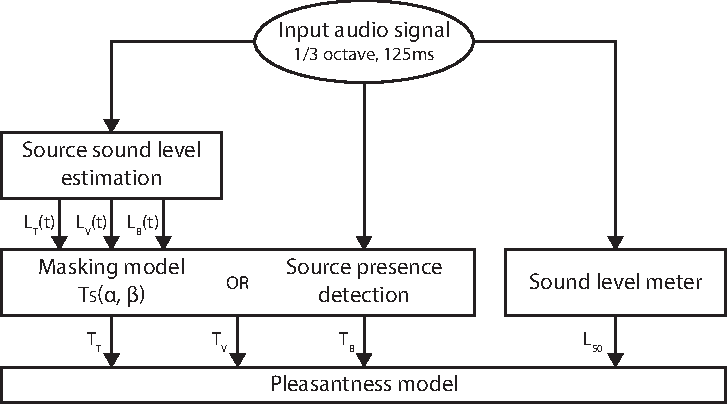
\includegraphics[width=0.8\textwidth]{figures/ppred.pdf}
    \caption{Processing chain applied to obtain an estimation of pleasantness in a recorded scene.}\label{fig:ppred}
\end{figure}

Based on the results outlined by the perceptual experiment, a processing chain is obtained for the estimation of pleasantness in urban sound scenes as shown in Figure~\ref{fig:ppred}. Pleasantness is modeled as a function of overall loudness and the perceived times of presence of traffic, voices and birds sources.

Predicting these quantities directly from audio recordings using deep learning architectures is difficult: training this type of models requires large annotated datasets which would require extensive work by several humans to obtain relevant labels. However, the perceived time of presence can be approximated by a simple masking model as demonstrated in Section~\ref{sec:physm}. While the same need for annotation of large datasets exists, it can be circumvented by the use of simulated data, for which the contribution of each source in the mix is available. Thus, a deep learning model can be used to predict either of the first steps of the pleasantness estimation chain.\\

An advantage of predicting sound levels is the accuracy of the labels as they are computed directly on available separated sources audio. Assuming that isolated samples used during scene generation are of good quality in terms of low other source content, the resulting ground truth labels can be considered as reliable. However, the prediction is a regression task which is typically difficult to learn. The best studied masking model relies on third-octave band sound levels, meaning that the learned model needs to perform an implicit source separation. Moreover, once an estimation of the sound levels are obtained the selected masking model must be used as the next step of pleasantness prediction. This model is not fully accurate and thus leads to small errors in pleasantness values even for perfect sound level estimations.\\

Instead, we can choose to directly predict if each of the three sources is present (heard) at a given time. This is either a detection problem if the data is processed asynchronously or a multi-label classification problem if the data is processed in frames, both of which are much simpler tasks. The corresponding labels are directly the outputs of the best studied masking model $\hat T(\alpha, \beta)$. Its uncertainties are thus transferred to "weak" labels rather than considered as part of the constant processing chain used to obtain pleasantness estimations.\\

In the following sections, two models for source-specific sound level and presence estimation are implemented and compared.

\subsection{Data}
\label{sec:pred_data}

Two datasets of simulated scenes are created for the proposed task:
\begin{itemize}
\item The development set containing 400 45~s scenes (total 5 hours) is used during the training process
\item The evaluation set containing 200 45~s scenes (total 2.5 hours) is used to compute the model's performance and its generalization capabilities
\end{itemize}

The generation procedure is the same for both datasets, and is equivalent to that of the simulated sub-corpus considered for the perceptual test. Only traffic, human voices and birds sources compose the sound scenes due to the low number of available samples for other sources. The isolated samples database is split in the same proportions as the two datasets: two-thirds for the development set and the remaining one-third for the evaluation set. As a result, while the generation process is the same for both corpora both the scenarios and samples are different.\\

The sensors implemented as part of the Cense project provide fast measurements of sound levels for each third-octave band in the $20~Hz - 12.5~kHz$ range in their normal operation~\cite{gontier2017}. Thus, the model should take as input the same representation. Third-octave spectra are computed for 125~ms frames and 29 frequency bands of the mixed sound scenes. Inputs are then obtained by splitting the resulting spectrograms into frames with a 1~s duration. This scale is considered relevant for perception and was already used to compute the masking models proposed in the perceptual experiment results analysis. The input frames of dimension 29x8 are processed independently in this study.\\

Target outputs differ for the level estimation and source detection. In the former case labels are obtained by computing the full-band sound level of source-specific audio channels. For the latter task the weak presence labels given by $\hat T(\alpha, \beta)$ before averaging along time are used. Estimates of pleasantness are obtained as follows:
\begin{itemize}
\item Sound level model: the outputs are used to compute the $\hat T(\alpha)$ indicator, which is then applied to equation (13),
\item Presence model: outputs are averaged along time and considered as $\hat T(\alpha, \beta)$ in equation (13).
\end{itemize}

\subsection{Model}
\label{sec:pred_mdl}

Deep learning models are implemented and trained separately for both sound level and presence prediction tasks, with architectures shown in Figure~\ref{fig:deep_arch}. For both tasks, the models include 4 blocks of convolutional layers followed by LeakyReLU activations. The convolutional layers have respectively 128, 64, 32 and 32 output maps (channels), and a common kernel size of 5x5. The output of the last block is flattened then goes through a fully connected layer with output size 3. For the model trained to predict sound levels these 3 values are taken directly as the model output, corresponding to the estimated level of traffic, voices and birds respectively. An additional sigmoid activation is added for the model predicting source presence to obtain outputs in the 0-1 range.

\begin{figure}[!h]
    \centering
    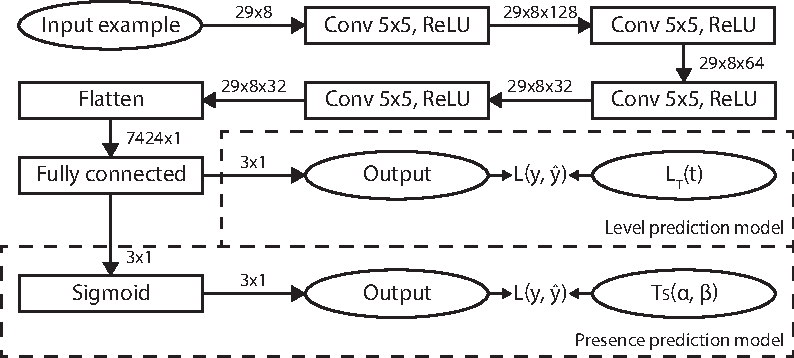
\includegraphics[width=0.8\textwidth]{figures/deep_arch.pdf}
    \caption{Architecture of deep learning models used for sound level or source presence prediction.}\label{fig:deep_arch}
\end{figure}

\subsection{Training details}

Training the models is achieved by progressively minimizing a loss function $L(y, \hat y)$, where $y$ and $\hat y$ represent the target and predicted outputs respectively. For sound level estimation we use the MSE or L2 loss:
\begin{equation}
L(y, \hat y) = \sum_s \left(\hat y_s - y_s\right)^2
\end{equation}
where $s$ is the source, $y_s$ and $\hat y_s$ are the target and predicted sound level of source $s$ in dB. For the prediction of the presence, the cost function is the binary cross-entropy of equation:
\begin{equation}
L(y, \hat y) = -\sum_s y_s log\left(\hat y_s\right) + (1-y_s) log\left(1-\hat y_s\right)
\end{equation}
where $s$ is the source, $y_s$ and $\hat y_s$ are the target and predicted presence for source $s$ in the 0-1 range.\\

Models are optimized using the Adam algorithm~\cite{kingma2015} on mini-batches of 64 1s examples. For all experiments a constant learning rate of $\lambda = 0.001$ is used. Training is performed during 10 epochs, that is iterations over the whole training set. As shown in Figure~\ref{fig:mdl_loss}, at that point the training loss is still decreasing but not the validation loss, indicating that the model starts overfitting the training data.

\begin{figure}[!h]
    \centering
    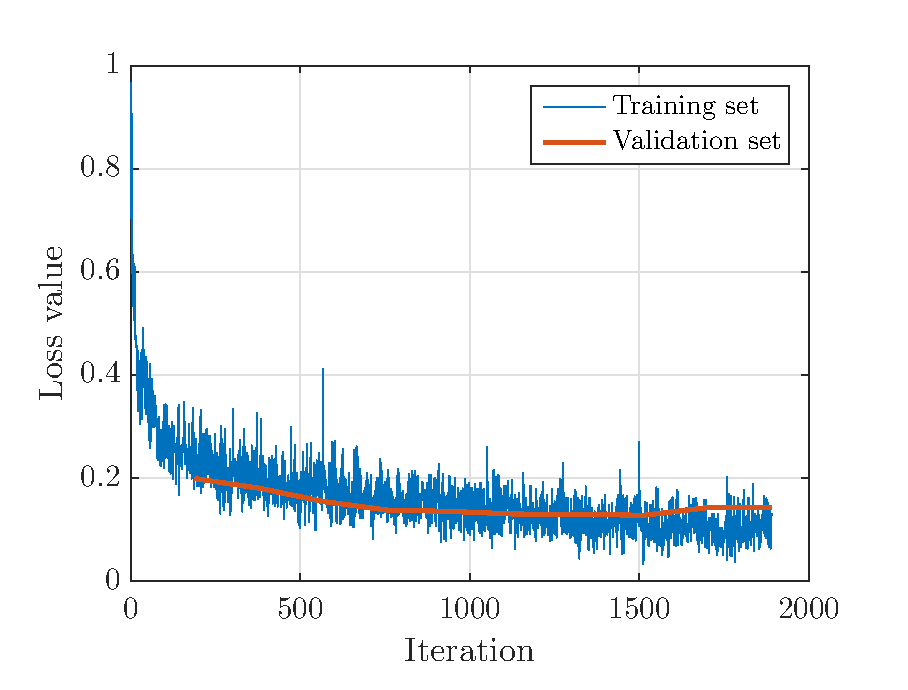
\includegraphics[width=0.8\textwidth]{figures/mdl_loss.eps}
    \caption{Evolution of the presence detection model's loss as a function of training iterations.}\label{fig:mdl_loss}
\end{figure}

\subsection{Metrics}

Performance metrics can be computed at either part of the processing chain shown in Figure~\ref{fig:ppred}. At the physical level, the following are considered:

\begin{itemize}
\item Sound level error for the sound level prediction model only as the presence prediction model bypasses this step,
\item Accuracy of source presence detection in 1~s frames with labels taken from the computation of $\hat T_s(\alpha, \beta)$ before averaging,
\item Error of the resulting time of presence with $\hat T_s(\alpha, \beta)$ as the assumed ground truth.
\end{itemize}

Additionally, the pleasantness estimates resulting from each model can be compared to assessments, although on the perceptual experiment corpus only as no subjective annotation was performed on the constructed evaluation dataset.

\subsection{Results}

Table~\ref{tab:perf_cmp} displays the performance of the two studied models for metrics at the physical level. The first model outputs very poor estimations of the source-specific sound level, but the resulting source presence accuracy is high at 92.51\%. As a result, the time of presence estimates are precise with a root mean square error of 0.12 on a 0-1 scale. This behavior may be explained by the fact that $\hat T_s(\alpha)$ indicator is too permissive: if some sources are close in terms of full-band sound level, the threshold $\alpha = -19dB$ allows rougher estimates for binary presence values. Thus, because the sound level model output is used in $\hat T_s(\alpha)$, there are two cases for which the correct presence is obtained
\begin{enumerate}
\item The model outputs very low level values for sources that are not present
\item The model outputs poor estimates but with sufficiently close values for all present sources
\end{enumerate}
Thus, the model may fail at the source separation and level estimation task and is here probably closer to a detection model.\\

The presence detection model performs well for both presence accuracy (92.11\%) and resulting $\hat T_s(\alpha, \beta)$ estimation (0.12 RMSE). Both models obtain lower accuracies for birds than for traffic or voices. However, the origin of errors varies. The sound level model has an very low false positive rate across sources while its false negative rate varies from 7.8\% for traffic to more than 18\% for birds. The opposite is observed for the presence model which displays a higher false positive rate for birds. Overall, traffic is found to be the source that is most easily detected. This may be due to its power spectral density that is concentrated in the lower frequency bands while voice and bird information is usually concentrated in narrower frequency ranges when using third-octave bands.\\


\begin{table}[t]
\centering
\caption{Comparison of performances of models predicting source sound level or presence with metrics at the physical level. Levels and presence metrics are computed for n=8600 1s frames and time of presence metrics on n=200 45s scenes. (TP: true positive, TN: true negative, FP: false positive, FN: false negative)}
\label{tab:perf_cmp}
\resizebox{\columnwidth}{!}{
\begin{tabular}{ c | c | c c c | c | c c c }
\hline
	Model & \multicolumn{4}{|c}{Sound level} & \multicolumn{4}{|c}{Presence} \\ \hline
	 & All sources & Traffic & Voices & Birds & All sources & Traffic & Voices & Birds \\ \hline
	Sound level RMSE (dB) & 12.91 & - & - & - & - & - & - & - \\
	Sound level MAE (dB) & 6.91 & - & - & - & - & - & - & - \\ \hline
	Presence accuracy (\%) & 92.51 & 93.65 & 92.90 & 90.98 & 92.11 & 94.09 & 92.15 & 90.08 \\
	Presence TP (\%) & 88.20 & 92.16 & 88.08 & 81.62 & 91.96 & 92.70 & 89.93 & 93.37 \\
	Presence TN (\%) & 97.86 & 97.34 & 98.32 & 97.74 & 92.30 & 97.54 & 94.76 & 87.70 \\
	Presenct FP (\%) & 2.14 & 2.66 & 1.68 & 2.26 & 7.70 & 2.46 & 5.24 & 12.30 \\
	Presence FN (\%) & 11.80 & 7.84 & 11.92 & 18.38 & 8.04 & 7.30 & 10.17 & 6.63 \\ \hline
	$\hat T_s(\alpha, \beta)$ RMSE & 0.12 & 0.14 & 0.11 & 0.12 & 0.12 & 0.13 & 0.10 & 0.11 \\
	$\hat T_s(\alpha, \beta)$ MAE & 0.06 & 0.06 & 0.06 & 0.07 & 0.06 & 0.05 & 0.06 & 0.08 \\ \hline
\end{tabular}
}
\end{table}

Next, a comparison is made of the models's capacity to result in relevant pleasantness estimates. For this analysis, the perceptual experiment is used as assessments are available. It is further split in two parts:
\begin{enumerate}
\item The 25 recorded and replicated scenes, which contain additional sources not present in the development or evaluation datasets simulated for the optimization of deep learning models,
\item The 75 simulated scenes that are obtained from the same simulation process as both the development and evaluation dataset.
\end{enumerate}
The results are shown in Table~\ref{tab:pppred}. Again, both models lead to similarly correct estimations of pleasantness with errors lower than 1.20 on a 10-point scale. Interestingly, predictions are better on the first tested sub-corpus which contains other sources, indicating that models are quite robust to this type of perturbation in the data. Though, a larger set of scenes and environments with perceptual annotations would be required to further validate this point.\\

The third part of Table~\ref{tab:pppred} refers to values of pleasantness obtained when using directly the $\hat T_s(\alpha, \beta)$ time of presence computed from ground truth separated channels (equation(13)). For the first sub-corpus only the 19 replicated scenes are used as the ground truth information is not available for the recorded part. For all the computed metrics the resulting error is higher than for both studied models. This is explained by the uncertainties of the $\hat T_s(\alpha, \beta)$ indicator that result from the simplicity of its masking model. The predictions from both models' outputs are in fact closer to the performance of the $\hat Pp3$ perceptual model presented in Section~\ref{sec:percm} (equation (3)).\\

Considering the abovementioned potential unstability of the sound level model, the presence detection model is to be preferred for further development.

\begin{table}[t]
\centering
\caption{Comparison of pleasantness prediction quality from predicted sound level and presence of sources. The experiment corpus is split into respectively the 25 recorded and replicated scenes and 75 simulated scenes.}
\label{tab:pppred}
%\resizebox{\columnwidth}{!}{
\begin{tabular}{ c | c c | c c | c c }
\hline
	Model & \multicolumn{2}{|c}{Sound level} & \multicolumn{2}{|c}{Presence} & \multicolumn{2}{|c}{$\hat T_s(\alpha, \beta)$} \\ \hline
	Sub-corpus & 1 & 2 & 1 & 2 & 1 & 2 \\ \hline
	RMSE & 1.02 & 1.17 & 1.12 & 1.18 & 1.33 & 1.29 \\
	MAE & 0.79 & 0.97 & 0.82 & 0.95 & 1.00 & 1.02 \\ \hline
	r & 0.85** & 0.79** & 0.86** & 0.80** & 0.76** & 0.77** \\ \hline
\end{tabular}
%}
\end{table}




\section{Conclusion}

A perceptual experiment is conducted with the objectives of 1) demonstrating that scenes replicated from annotations of recordings yield similar perceptual responses to these recordings, 2) simulated scenes with new scenarios can be used to develop perceptual models, 3) physical indicators can be computed from audio signals from which pleasantness can be efficiently predicted. These three hypotheses are verified, and a pleasantness model relying on presence detection for traffic, voices and bird sources is proposed.\\

Subsequently, a deep learning model with state-of-the-art architecture is developed for this task. The model takes as input the fast third-octave band representation of the mixed scene and is trained on a corpus of simulated scenes to output presence labels in short time frames of 1s. Low pleasantness prediction errors are achieved on the perceptual experiment corpus: around 1.15 root mean square error on the 10-point scale which is below the mean standard deviation of pleasantness assessments of 1.77.\\

Future work will focus on the study of the robustness of developed models to new environment and data. Here only three sources were considered during training, and a limited isolated sound sources database have been considered. Thus, pleasantness estimation chain needs to be evaluated using data gathered in the experimentation site, where the Cense sensor network is to be implemented.


\clearpage




%\begin{itemize}
%\item
%\item
%\item
%\end{itemize}


%\begin{table}
%\centering
%\caption{}
%\label{tab:}
%%\resizebox{\columnwidth}{!}{
%\begin{tabular}{ c | c c c c c c c c c }
%\hline
%	 & P & L & OL & I & C & $V_{V, p}$ & $T_{T, p}$ & $T_{V, p}$ & $T_{B, p}$ \\ \hline
%	P1 &  &  &  &  &  &  &  &  &  \\
%	P3 &  &  &  &  &  &  &  &  &  \\
%	P4 &  &  &  &  &  &  &  &  &  \\
%	P8 &  &  &  &  &  &  &  &  &  \\
%	P15 &  &  &  &  &  &  &  &  &  \\
%	P18 &  &  &  &  &  &  &  &  &  \\ \hline
%\end{tabular}
%%}
%\end{table}

\bibliographystyle{plain}
\bibliography{refs}

\end{document}
